\documentclass{article}
\usepackage{../assignment_preamble}

\title{Homework 5}
\author{Ravi Kini}
\date{November 26, 2025}

\begin{document}

\maketitle

\problem{}
\subproblem{(a)}
\begin{align*}
    A = \begin{bmatrix}
        -5 \\ 3
    \end{bmatrix}
\end{align*}
To compute the SVD decomposition of $A$, we first find the eigenvalues of $AA^T$.
\begin{align*}
    AA^T & = \begin{bmatrix}
        25 & -15 \\ -15 & 9
    \end{bmatrix} \\
    \lambda & = 0, 34 \\
    \sigma_1 & = \sqrt{34}
\end{align*}
The corresponding unit eigenvectors, which are the columns of $V$, are:
\begin{align*}
    \begin{bmatrix}
        25 & -15 \\ -15 & 9
    \end{bmatrix}v_1 & = 34v_1 \\
    v_1 & = \frac{1}{\sqrt{34}}\begin{bmatrix}
        -5 \\ 3
    \end{bmatrix} \\
    \begin{bmatrix}
        25 & -15 \\ -15 & 9
    \end{bmatrix}v_2 & = 0v_2 \\
    v_2 & = \frac{1}{\sqrt{34}}\begin{bmatrix}
        3 \\ 5
    \end{bmatrix}
\end{align*}
The columns of $U$ are then:
\begin{align*}
    u_1 & = \frac{1}{\sigma_1}A^Tv_1 = \begin{bmatrix}
        1
    \end{bmatrix}
\end{align*}
The SVD decomposition is then:
\begin{align*}
    A & = \begin{bmatrix}
        -5/\sqrt{34} & 3/\sqrt{34} \\ 3/\sqrt{34} & 5/\sqrt{34}
    \end{bmatrix}\begin{bmatrix}
        \sqrt{34} \\ 0
    \end{bmatrix}\begin{bmatrix}
        1
    \end{bmatrix}^T
\end{align*}
\subproblem{(b)}
\begin{align*}
    A = \begin{bmatrix}
        1 & 2 \\ 2 & 2 \\ 2 & 1
    \end{bmatrix}
\end{align*}
To compute the SVD decomposition of $A$, we first find the eigenvalues of $AA^T$.
\begin{align*}
    AA^T & = \begin{bmatrix}
        5 & 6 & 4 \\ 6 & 8 & 6 \\ 4 & 6 & 5
    \end{bmatrix} \\
    \lambda & = 0, 1, 17 \\
    \sigma_1 & = \sqrt{17} \\
    \sigma_2 & = 1
\end{align*}
The corresponding unit eigenvectors, which are the columns of $V$, are:
\begin{align*}
    \begin{bmatrix}
        5 & 6 & 4 \\ 6 & 8 & 6 \\ 4 & 6 & 5
    \end{bmatrix}v_1 & = 17v_1 \\
    v_1 & = \frac{1}{\sqrt{34}}\begin{bmatrix}
        3 \\ 4 \\ 3
    \end{bmatrix} \\
    \begin{bmatrix}
        5 & 6 & 4 \\ 6 & 8 & 6 \\ 4 & 6 & 5
    \end{bmatrix}v_2 & = 1v_2 \\
    v_2 & = \frac{1}{\sqrt{2}}\begin{bmatrix}
        -1 \\ 0 \\ 1
    \end{bmatrix} \\
    \begin{bmatrix}
        5 & 6 & 4 \\ 6 & 8 & 6 \\ 4 & 6 & 5
    \end{bmatrix}v_3 & = 0v_3 \\
    v_3 & = \frac{1}{\sqrt{17}}\begin{bmatrix}
        2 \\ -3 \\ 2
    \end{bmatrix}
\end{align*}
The columns of $U$ are then:
\begin{align*}
    u_1 & = \frac{1}{\sigma_1}A^Tv_1 = \frac{1}{\sqrt{2}}\begin{bmatrix}
        1 \\ 1
    \end{bmatrix} \\
    u_2 & = \frac{1}{\sigma_2}A^Tv_2 = \frac{1}{\sqrt{2}}\begin{bmatrix}
        1 \\ -1
    \end{bmatrix}
\end{align*}
The SVD decomposition is then:
\begin{align*}
    A & = \begin{bmatrix}
        3/\sqrt{34} & -1/\sqrt{2} & 2/\sqrt{17} \\ 4/\sqrt{34} & 0 & 1/\sqrt{2} \\ 2/\sqrt{17} & -3/\sqrt{17} & 2/\sqrt{17}
    \end{bmatrix}\begin{bmatrix}
        \sqrt{17} & 0 \\ 0 & 1 \\ 0 & 0 
    \end{bmatrix}\begin{bmatrix}
        1/\sqrt{2} & 1/\sqrt{2} \\ 1/\sqrt{2} & -1/\sqrt{2}
    \end{bmatrix}^T
\end{align*}
\subproblem{(c)}
\begin{align*}
    A = \begin{bmatrix}
        0 & 0 & 1 \\ 0 & \sqrt{2} & 0 \\ 3 & 0 & 0
    \end{bmatrix}
\end{align*}
To compute the SVD decomposition of $A$, we first find the eigenvalues of $AA^T$.
\begin{align*}
    AA^T & = \begin{bmatrix}
        1 & 0 & 0 \\ 0 & 2 & 0 \\ 0 & 0 & 3
    \end{bmatrix} \\
    \lambda & = 1, 2, 3 \\
    \sigma_1 & = \sqrt{3} \\
    \sigma_2 & = \sqrt{2} \\
    \sigma_3 & = 1
\end{align*}
The corresponding unit eigenvectors, which are the columns of $V$, are:
\begin{align*}
    \begin{bmatrix}
        1 & 0 & 0 \\ 0 & 2 & 0 \\ 0 & 0 & 3
    \end{bmatrix}v_1 & = 3v_1 \\
    v_1 & = \begin{bmatrix}
        0 \\ 0 \\ 1
    \end{bmatrix} \\
    \begin{bmatrix}
        1 & 0 & 0 \\ 0 & 2 & 0 \\ 0 & 0 & 3
    \end{bmatrix}v_2 & = 2v_2 \\
    v_2 & = \begin{bmatrix}
        0 \\ 1 \\ 0
    \end{bmatrix} \\
    \begin{bmatrix}
        1 & 0 & 0 \\ 0 & 2 & 0 \\ 0 & 0 & 3
    \end{bmatrix}v_3 & = 1v_3 \\
    v_3 & = \begin{bmatrix}
        1 \\ 0 \\ 0
    \end{bmatrix}
\end{align*}
The columns of $U$ are then:
\begin{align*}
    u_1 & = \frac{1}{\sigma_1}A^Tv_1 = \frac{1}{\sqrt{3}}\begin{bmatrix}
        1 \\ 0 \\ 0
    \end{bmatrix} \\
    u_2 & = \frac{1}{\sigma_2}A^Tv_2 = \begin{bmatrix}
        0 \\ 1 \\ 0
    \end{bmatrix} \\
    u_3 & = \frac{1}{\sigma_3}A^Tv_3 = \sqrt{3}\begin{bmatrix}
        0 \\ 0 \\ 1
    \end{bmatrix}
\end{align*}
The SVD decomposition is then:
\begin{align*}
    A & = \begin{bmatrix}
        1/\sqrt{3} & 0 & 0 \\ 0 & 1 & \sqrt{3} \\ 
    \end{bmatrix}\begin{bmatrix}
        \sqrt{3} & 0 & 0 \\ 0 & \sqrt{2} & 0 \\ 0 & 0 & 1 
    \end{bmatrix}\begin{bmatrix}
        0 & 0 & 1 \\ 0 & 1 & 0 \\ 1 & 0 & 0
    \end{bmatrix}^T
\end{align*}

\clearpage
\problem{}
Let $A = ab^T$ where $a \in \mathbb{R}^m$ and $b \in \mathbb{R}^n$.
\subproblem{(a)}
We see that:
\begin{align*}
    AA^T & = ab^T{(ab^T)}^T \\
    & = ab^Tba^T = (b^Tb)aa^T \\
    & = ||b||^2 aa^T
\end{align*}
We see that this matrix has eigenvalue $\sigma_1^2 = ||a||^2||b||^2$, with corresponding eigenvector $v_1 = b/||b||_2$. Then $u_1 = \frac{1}{\sigma_1}Av_1 = a/||a||_2$. The largest singular triplet is $(||a||||b||, a/||a||_2, b/||b||_2)$.
\subproblem{(b)}
Consequently, $||A||_2 = \sigma_1 = ||a||||b||$ and $||A||_F = \sqrt{\mathrm{tr}(AA^T)} = \sqrt{||b||^2\mathrm{tr}(aa^T)} = \sqrt{||b||^2||a||^2} = ||a||||b||$.

\clearpage
\problem{}
Let $A$ be a symmetric $n \times n$ matrix. It then has the spectral decomposition $A = Q\Lambda Q^T$ where $Q$ is orthogonal and $\Lambda$ is diagonal. Then:
\begin{align*}
    AA^T & = (Q\Lambda Q^T)(Q\Lambda Q^T)^T \\
    & = Q\Lambda Q^TQ\Lambda Q^T \\
    & = Q\Lambda^2 Q^T
\end{align*}
The SVD decomposition of $A$ then has $U = Q$, $\Sigma = \Lambda^2$, and $V = Q$.

\clearpage
\problem{}
Let $A$ be nonsingular, with singular values $\sigma_1 \geq \ldots \geq \sigma_n > 0$ and SVD decomposition $U\Sigma V^T$.
\subproblem{(a)}
To find the SVD decomposition of $A^{-1}$:
\begin{align*}
    A^{-1} & = {(U\Sigma V^T)}^{-1} \\
    & = {(V^T)}^{-1}\Sigma^{-1} U^{-1}
\end{align*}
Since $U$ and $V$ are orthogonal:
\begin{align*}
    A^{-1} & = V^T\Sigma U
\end{align*}
where $\Sigma^{-1} = \mathrm{diag}(\sigma_1, \ldots, \sigma_n)$.
\subproblem{(b)}
The singular values of $A^{-1}$ are the inverses of the singular values of $A$. The left singular vectors of $A^{-1}$ are the right singular vectors of $A$ and vice versa.
\subproblem{(c)}
Since the $2$-norm is equal to the largest singular value, $||A^{-1}||_2 = 1/\sigma_n$.
\subproblem{(d)}
Since $||A||_2 = \sigma_1$, we see that $\mathrm{cond}(A) = ||A||_2 \cdot ||A^{-1}||_2 = \sigma_1/\sigma_n$.

\clearpage
\problem{}
Let $A$ be a $n \times n$ matrix with SVD decomposition $U\Sigma V^T$. Then:
\begin{align*}
    A^TA & = {(U\Sigma V^T)}^T(U\Sigma V^T) \\
    & = (V\Sigma U^T)(U\Sigma V^T) \\
    & = V\Sigma^2 V^T
\end{align*}
The singular values of $A^TA$ are then the squares of the singular values of $A$. Further, since $A^TA$ is symmetric, the singular values of ${(A^TA)}^{-1}$ are the inverses of the singular values of $A^TA$. Consequently, $\mathrm{cond}(A^TA) = ||A^TA||_2 \cdot ||{(A^TA)}^{-1}||_2 = \sigma_1^2/\sigma_n^2$.

\clearpage
\problem{}
Let $f(x) = \frac{1}{x} - a$, which has a root at $x = \frac{1}{a}$.
\subproblem{(a)}
Since $f'(x) = - \frac{1}{x^2}$, the Newton iteration is:
\begin{align*}
    x_{k+1} & = x_k - \frac{f(x_k)}{f'(x_k)} \\
    & = x_k - \frac{\frac{1}{x_k} - a}{- \frac{1}{x_k^2}} \\
    & = x_k + (x_k - ax_k^2) = 2x_k - ax_k^2
\end{align*}
\subproblem{(b)}
With an initial guess of $x_0 = 0.5$ and $a = 3$, the first four Newton iterations are:
\begin{center}
\begin{tabular}{|c|c|}
    \hline
    $k$ & $x_k$ \\
    \hline
    $1$ & $2 \cdot 0.5 - 3 \cdot 0.5^2 = 0.25$ \\
    \hline
    $2$ & $2 \cdot 0.25 - 3 \cdot 0.25^2 = 0.3125$ \\
    \hline
    $3$ & $2 \cdot 0.3125 - 3 \cdot 0.3125^2 \approx 0.3320$ \\
    \hline
    $4$ & $2 \cdot 0.3320 - 3 \cdot 0.3320^2 = 0.3333$ \\
    \hline
\end{tabular}
\end{center}
\subproblem{(c)}
Let $e_k = ax_k - 1$, where $x_k$ is the $k$th approximation using Newton's method. Then:
\begin{align*}
    e_{k+1} & = ax_{k+1} - 1 \\
    & = a(2x_k - ax_k^2) - 1 = -(a^2x_k^2 - 2ax_k + 1) = -e_k^2\\
\end{align*}
\subproblem{(d)}
For Newton's method to converge, we require that $|e_{k+1}| < |e_k|$. Since $e_{k+1} = -e_k^2$, this implies that $|e_k|^2 < |e_k|$, and so $|e_k| < 1$. This means that the initial guess $x_0$ must satisfy:
\begin{align*}
    |ax_0 - 1| & < 1 \\
    -1 < ax_0 - 1 & < 1 \\
    0 < ax_0 & < 2 \\
    0 < x_0 & < \frac{2}{a} \\
\end{align*}

\clearpage
\problem{}
\begin{align*}
    p(x) = 816x^3 - 3835x^2 + 6000x - 3125
\end{align*}
\subproblem{(a)}
Plotting $p(x)$:
\begin{center}
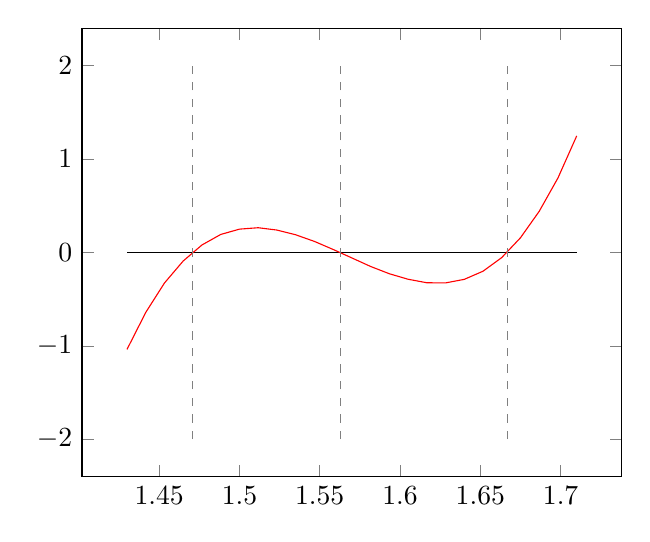
\begin{tikzpicture}
\begin{axis}
\addplot[domain=1.43:1.71,color=black]{0};
\addplot[domain=1.43:1.71,color=red]{816*x^3-3835*x^2+6000*x-3125};
\addplot[dashed,color=gray,mark=none] coordinates {(1.667,-2) (1.667,2)};
\addplot[dashed,color=gray,mark=none] coordinates {(1.563,-2) (1.563,2)};
\addplot[dashed,color=gray,mark=none] coordinates {(1.471,-2) (1.471,2)};
\end{axis}
\end{tikzpicture}
\end{center}
\subproblem{(b)}
\begin{lstlisting}[language=Python]
EPS = 2.2e-16

def bisection(f, a, b):
    if f(a) * f(b) > 0:
        return None
    i = 0
    c = (a + b) / 2
    while abs(f(c)) > EPS:
        c = (a + b) / 2
        i += 1
        if f(a) * f(c) > 0:
            a = c
        else:
            b = c
    return c, i

p = lambda x : 816 * x ** 3 - 3835 * x ** 2 + 6000 * x - 3125
print(bisection(p, 1, 2))
\end{lstlisting}
Starting with the interval $[a, b] = [1, 2]$, the bisection method converges to the root $x = \frac{25}{17}$ in $41$ iterations.
\subproblem{(c)}
\begin{lstlisting}[language=Python]
EPS = 2.2e-16

def newton(f, f_p, x_0):
    i = 0
    x = x_0 - f(x_0) / f_p(x_0)
    while abs(f(x)) > EPS:
        i += 1
        x = x - f(x) / f_p(x)
    return x, i

p = lambda x : 816 * x ** 3 - 3835 * x ** 2 + 6000 * x - 3125
p_ = lambda x : 816 * 3 * x ** 2 - 3835 * 2 * x + 6000
print(newton(p, p_, 1.5))
\end{lstlisting}
Starting with the initial guess $x_0 = 1.5$, Newton's method converges to the root $x = \frac{25}{17}$ in $7$ iterations.
\subproblem{(d)}
\begin{lstlisting}[language=Python]
EPS = 2.2e-16

def secant(f, x_0, x_1):
    i = 0
    x, x_prev = x_1 - f(x_1) * (x_1 - x_0) / (f(x_1) - f(x_0)), x_1
    while abs(f(x)) > EPS:
        i += 1
        x, x_prev = x - f(x) * (x - x_prev) / (f(x) - f(x_prev)), x
    return x, i

p = lambda x : 816 * x ** 3 - 3835 * x ** 2 + 6000 * x - 3125
print(secant(p, 1, 2))
\end{lstlisting}
Starting with the initial guesses $x_0 = 1$ and $x_1 = 2$, the secant method converges to the root $x = \frac{25}{15}$ in $10$ iterations.

\clearpage
\problem{}
\begin{align*}
    f(x) = \mathrm{sign}(x - 2)\sqrt{|x - 2}
\end{align*}
\begin{lstlisting}[language=Python]
EPS = 2.2e-16

sign = lambda x : 1 if x > 0 else -1 if x < 0 else 0

def secant(f, x_0, x_1):
    i = 0
    x, x_prev = x_1 - f(x_1) * (x_1 - x_0) / (f(x_1) - f(x_0)), x_1
    while abs(f(x)) > EPS:
        i += 1
        x, x_prev = x - f(x) * (x - x_prev) / (f(x) - f(x_prev)), x
    return x, i

p = lambda x : sign(x - 2) * abs(x - 2) ** 0.5
print(secant(p, 0, 1))
\end{lstlisting}
Starting with the initial guesses $x_0 = 0$ and $x_1 = 1$, the secant method converges to the root $x = 2$ in $73$ iterations.
\end{document}